% !TEX encoding = UTF-8
% !TEX TS-program = pdflatex
% !TEX root = relazione.tex
% !TEX spellcheck = it-IT
\subsection{Pagina interna - Articolo}
\label{sub:articolo}
Anche in questo caso, le pagine degli articoli tendono a essere molto lunghe, per cui si consiglia di visualizzare il file \href{pic/articolo.jpeg}{\underline{articolo.jpeg}} (o di cliccare sull'immagine qui raffigurata).
\begin{figure}[h]
\centering
\href{pic/articolo.jpeg}{
\includegraphics[height=0.5\textheight]{articolo}}
\caption{\href{pic/articolo.jpeg}{Pagina interna - articolo}} % http://www.nintendolife.com/news/2017/05/nintendo_download_4th_may_europe
\end{figure}

\subsubsection{Struttura}
\label{sub:articolo-struttura}
Le pagine interne di articoli seguono tutte la stessa struttura, che è come segue:
\begin{itemize}
    \item \emph{Header} e \emph{Footer} identici a prima
    \item Sotto il primo banner pubblicitario, il contenuto comincia con una lista di \textbf{etichette} che denotano gli argomenti attinenti all'articolo corrente (ogni articolo ha delle etichette associate)
    \item Sotto il breadcrumb, viene ripreso il titolo e il \emph{blurb} visti anche nella homepage; è riportato inoltre il nome dell'autore dell'articolo, e a destra sono presenti pulsanti appositi per la condivisione su social network
    \item L'immagine immediatamente sotto è sempre presente (può essere rimpiazzata da un video) e generalmente è la versione completa della \emph{thumbnail} dell'articolo nella home
    \item Sotto comincia l'articolo vero e proprio
    \item Caso particolare di quest'articolo, è presente anche un sondaggio alla fine del testo
    \item Dopo il sondaggio c'è una lista di giochi correlati all'articolo
    \item Segue una griglia di banner pubblicitari che riprendono lo stile degli articoli nella homepage
    \item Dopo la pubblicità c'è la sezione commenti; in fondo alla lista è possibile, se registrati, inserire il proprio commento
    \item A sinistra della sezione commenti c'è una breve descrizione dell'autore e una lista di articoli correlati
    \item Nella sidebar a destra vi è una lista dei giochi menzionati nell'articolo che segue lo scroll della pagina.
\end{itemize}
Le recensioni dei giochi hanno due elementi aggiuntivi (fig.\ref{fig:recensione}): il voto assegnato al gioco e una ``finestra'' a destra che contiene le informazioni del titolo in esame. La finestra segue lo scroll dell'utente.
\begin{figure}[h]
    \centering
    \href{pic/recensione.jpeg}{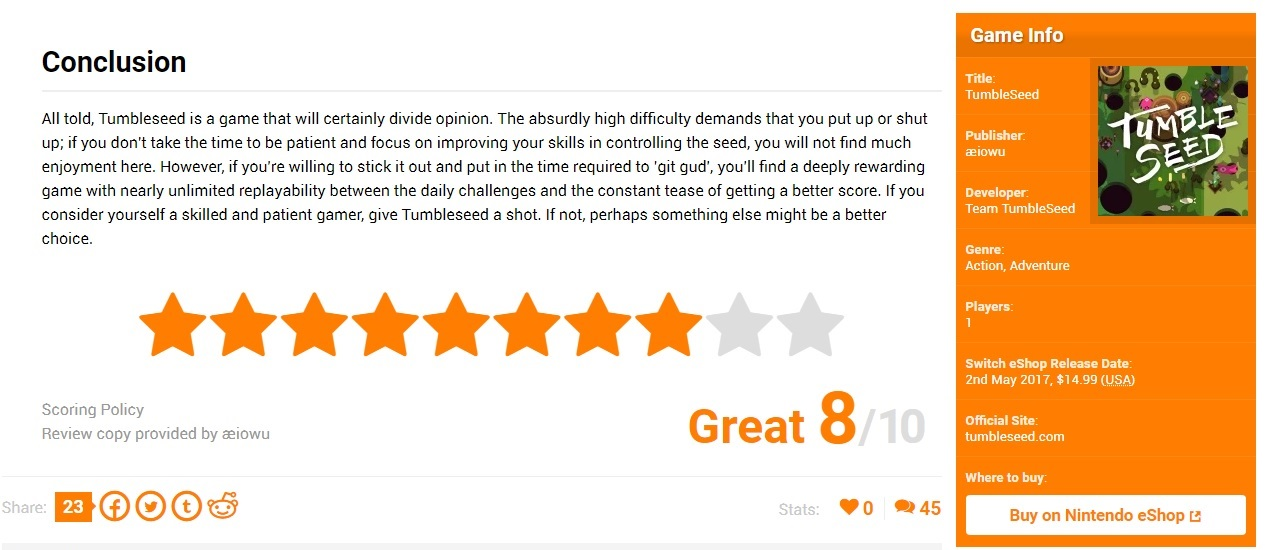
\includegraphics[width=\textwidth]{recensione}}
    \caption{\href{pic/recensione.jpeg}{Elementi aggiuntivi di una recensione}\label{fig:recensione}} % http://www.nintendolife.com/reviews/switch-eshop/tumbleseed#conclusion
\end{figure}

\subsubsection{Analisi}
\label{sub:articolo-analisi}
Anche in questo caso, la pagina rimane troppo lunga \xmark e il testo dell'articolo viene spinto troppo in basso dall'immagine: è probabile che l'utente sia costretto ad effettuare uno scroll per iniziare a leggerlo \xmark.\\
Essendo una pagina interna, non è necessario che tutti gli assi informativi siano sviluppati. Gli unici assi che rimangono obbligatori sono \textbf{Who} e \textbf{What}:
\begin{description}
    \item[Who] \hfill \\ Come nella homepage, le uniche informazioni a riguardo sono nel footer, quindi richiedono molto scroll per essere viste \xmark
    \item[What] \hfill \\ Rimane visibile la barra di navigazione, che mostra sinteticamente l'offerta del sito \cmark; inoltre, l'utente può passare sopra ai relativi pulsanti con il mouse per aprire i menu di navigazione, che forniscono ulteriori dettagli \cmark
\end{description}
Per quanto riguarda gli altri assi, sono state fatte le seguenti osservazioni:
\begin{description}
    \item[Where] \hfill \\ Poiché gli articoli non sono organizzati in una gerarchia, non ha senso utilizzare un breadcrumb per orientare l'utente: l'unico livello superiore nella gerarchia è sempre la homepage, accessibile cliccando il logo o l'icona relativa nella barra di navigazione \cmark; inoltre, la lista di etichette aiuta l'utente a capire a che tipologia di articolo è arrivato \cmark
    \item[Why] \hfill \\ I pulsanti della barra di navigazione continuano a mostrare all'utente che cosa offre il sito \cmark
    \item[When] \hfill \\ La lista degli articoli correlati mostra le notizie più recenti su argomenti analoghi alla pagina corrente \cmark
\end{description}